% Options for packages loaded elsewhere
% Options for packages loaded elsewhere
\PassOptionsToPackage{unicode}{hyperref}
\PassOptionsToPackage{hyphens}{url}
\PassOptionsToPackage{dvipsnames,svgnames,x11names}{xcolor}
%
\documentclass[
]{report}
\usepackage{xcolor}
\usepackage{amsmath,amssymb}
\setcounter{secnumdepth}{5}
\usepackage{iftex}
\ifPDFTeX
  \usepackage[T1]{fontenc}
  \usepackage[utf8]{inputenc}
  \usepackage{textcomp} % provide euro and other symbols
\else % if luatex or xetex
  \usepackage{unicode-math} % this also loads fontspec
  \defaultfontfeatures{Scale=MatchLowercase}
  \defaultfontfeatures[\rmfamily]{Ligatures=TeX,Scale=1}
\fi
\usepackage{lmodern}
\ifPDFTeX\else
  % xetex/luatex font selection
\fi
% Use upquote if available, for straight quotes in verbatim environments
\IfFileExists{upquote.sty}{\usepackage{upquote}}{}
\IfFileExists{microtype.sty}{% use microtype if available
  \usepackage[]{microtype}
  \UseMicrotypeSet[protrusion]{basicmath} % disable protrusion for tt fonts
}{}
\makeatletter
\@ifundefined{KOMAClassName}{% if non-KOMA class
  \IfFileExists{parskip.sty}{%
    \usepackage{parskip}
  }{% else
    \setlength{\parindent}{0pt}
    \setlength{\parskip}{6pt plus 2pt minus 1pt}}
}{% if KOMA class
  \KOMAoptions{parskip=half}}
\makeatother
% Make \paragraph and \subparagraph free-standing
\makeatletter
\ifx\paragraph\undefined\else
  \let\oldparagraph\paragraph
  \renewcommand{\paragraph}{
    \@ifstar
      \xxxParagraphStar
      \xxxParagraphNoStar
  }
  \newcommand{\xxxParagraphStar}[1]{\oldparagraph*{#1}\mbox{}}
  \newcommand{\xxxParagraphNoStar}[1]{\oldparagraph{#1}\mbox{}}
\fi
\ifx\subparagraph\undefined\else
  \let\oldsubparagraph\subparagraph
  \renewcommand{\subparagraph}{
    \@ifstar
      \xxxSubParagraphStar
      \xxxSubParagraphNoStar
  }
  \newcommand{\xxxSubParagraphStar}[1]{\oldsubparagraph*{#1}\mbox{}}
  \newcommand{\xxxSubParagraphNoStar}[1]{\oldsubparagraph{#1}\mbox{}}
\fi
\makeatother


\usepackage{longtable,booktabs,array}
\usepackage{calc} % for calculating minipage widths
% Correct order of tables after \paragraph or \subparagraph
\usepackage{etoolbox}
\makeatletter
\patchcmd\longtable{\par}{\if@noskipsec\mbox{}\fi\par}{}{}
\makeatother
% Allow footnotes in longtable head/foot
\IfFileExists{footnotehyper.sty}{\usepackage{footnotehyper}}{\usepackage{footnote}}
\makesavenoteenv{longtable}
\usepackage{graphicx}
\makeatletter
\newsavebox\pandoc@box
\newcommand*\pandocbounded[1]{% scales image to fit in text height/width
  \sbox\pandoc@box{#1}%
  \Gscale@div\@tempa{\textheight}{\dimexpr\ht\pandoc@box+\dp\pandoc@box\relax}%
  \Gscale@div\@tempb{\linewidth}{\wd\pandoc@box}%
  \ifdim\@tempb\p@<\@tempa\p@\let\@tempa\@tempb\fi% select the smaller of both
  \ifdim\@tempa\p@<\p@\scalebox{\@tempa}{\usebox\pandoc@box}%
  \else\usebox{\pandoc@box}%
  \fi%
}
% Set default figure placement to htbp
\def\fps@figure{htbp}
\makeatother


% definitions for citeproc citations
\NewDocumentCommand\citeproctext{}{}
\NewDocumentCommand\citeproc{mm}{%
  \begingroup\def\citeproctext{#2}\cite{#1}\endgroup}
\makeatletter
 % allow citations to break across lines
 \let\@cite@ofmt\@firstofone
 % avoid brackets around text for \cite:
 \def\@biblabel#1{}
 \def\@cite#1#2{{#1\if@tempswa , #2\fi}}
\makeatother
\newlength{\cslhangindent}
\setlength{\cslhangindent}{1.5em}
\newlength{\csllabelwidth}
\setlength{\csllabelwidth}{3em}
\newenvironment{CSLReferences}[2] % #1 hanging-indent, #2 entry-spacing
 {\begin{list}{}{%
  \setlength{\itemindent}{0pt}
  \setlength{\leftmargin}{0pt}
  \setlength{\parsep}{0pt}
  % turn on hanging indent if param 1 is 1
  \ifodd #1
   \setlength{\leftmargin}{\cslhangindent}
   \setlength{\itemindent}{-1\cslhangindent}
  \fi
  % set entry spacing
  \setlength{\itemsep}{#2\baselineskip}}}
 {\end{list}}
\usepackage{calc}
\newcommand{\CSLBlock}[1]{\hfill\break\parbox[t]{\linewidth}{\strut\ignorespaces#1\strut}}
\newcommand{\CSLLeftMargin}[1]{\parbox[t]{\csllabelwidth}{\strut#1\strut}}
\newcommand{\CSLRightInline}[1]{\parbox[t]{\linewidth - \csllabelwidth}{\strut#1\strut}}
\newcommand{\CSLIndent}[1]{\hspace{\cslhangindent}#1}



\setlength{\emergencystretch}{3em} % prevent overfull lines

\providecommand{\tightlist}{%
  \setlength{\itemsep}{0pt}\setlength{\parskip}{0pt}}



 


% Required packages
\usepackage{graphicx}
\usepackage{geometry}
\usepackage{fancyhdr}
\usepackage{titling}
\usepackage{array}
\usepackage{booktabs}
\usepackage{xcolor}
\usepackage{hyperref}
\usepackage{setspace}
\usepackage{microtype}

% Better typography
\usepackage[protrusion=true,expansion=true]{microtype}

% Spacing
\onehalfspacing

% Header and footer styling
\pagestyle{fancy}
\fancyhf{}
\fancyhead[LE,RO]{\slshape\nouppercase{\rightmark}}
\fancyhead[LO,RE]{\slshape\nouppercase{\leftmark}}
\fancyfoot[C]{\thepage}
\makeatletter
\@ifpackageloaded{caption}{}{\usepackage{caption}}
\AtBeginDocument{%
\ifdefined\contentsname
  \renewcommand*\contentsname{Table of contents}
\else
  \newcommand\contentsname{Table of contents}
\fi
\ifdefined\listfigurename
  \renewcommand*\listfigurename{List of Figures}
\else
  \newcommand\listfigurename{List of Figures}
\fi
\ifdefined\listtablename
  \renewcommand*\listtablename{List of Tables}
\else
  \newcommand\listtablename{List of Tables}
\fi
\ifdefined\figurename
  \renewcommand*\figurename{Figure}
\else
  \newcommand\figurename{Figure}
\fi
\ifdefined\tablename
  \renewcommand*\tablename{Table}
\else
  \newcommand\tablename{Table}
\fi
}
\@ifpackageloaded{float}{}{\usepackage{float}}
\floatstyle{ruled}
\@ifundefined{c@chapter}{\newfloat{codelisting}{h}{lop}}{\newfloat{codelisting}{h}{lop}[chapter]}
\floatname{codelisting}{Listing}
\newcommand*\listoflistings{\listof{codelisting}{List of Listings}}
\makeatother
\makeatletter
\makeatother
\makeatletter
\@ifpackageloaded{caption}{}{\usepackage{caption}}
\@ifpackageloaded{subcaption}{}{\usepackage{subcaption}}
\makeatother
\usepackage{bookmark}
\IfFileExists{xurl.sty}{\usepackage{xurl}}{} % add URL line breaks if available
\urlstyle{same}
\hypersetup{
  pdftitle={Automating the Modelling of Transformative Artificial Intelligence Risks},
  pdfauthor={Valentin Jakob Meyer; Prof.~Dr.~Timo Speith},
  pdfkeywords={AMTAIR, AI Governance, Bayesian Networks, Transformative
AI, Risk Assessment, Argument Extraction},
  colorlinks=true,
  linkcolor={blue},
  filecolor={Maroon},
  citecolor={Blue},
  urlcolor={Blue},
  pdfcreator={LaTeX via pandoc}}


\title{Automating the Modelling of Transformative Artificial
Intelligence Risks}
\usepackage{etoolbox}
\makeatletter
\providecommand{\subtitle}[1]{% add subtitle to \maketitle
  \apptocmd{\@title}{\par {\large #1 \par}}{}{}
}
\makeatother
\subtitle{An Epistemic Framework for Leveraging Frontier AI Systems to
Upscale Conditional Policy Assessments in Bayesian Networks on a Narrow
Path towards Existential Safety}
\author{Valentin Jakob Meyer \and Prof.~Dr.~Timo Speith}
\date{2025-05-26}
\begin{document}
\maketitle
\begin{abstract}
The coordination crisis in AI governance presents a paradoxical
challenge: unprecedented investment in AI safety coexists alongside
fundamental coordination failures across technical, policy, and ethical
domains. These divisions systematically increase existential risk by
creating safety gaps, misallocating resources, and fostering
inconsistent approaches to interdependent problems. This thesis
introduces AMTAIR (Automating Transformative AI Risk Modeling), a
computational approach that addresses this coordination failure by
automating the extraction of probabilistic world models from AI safety
literature using frontier language models.

The AMTAIR system implements an end-to-end pipeline that transforms
unstructured text into interactive Bayesian networks through a novel
two-stage extraction process: first capturing argument structure in
ArgDown format, then enhancing it with probability information in
BayesDown. This approach bridges communication gaps between stakeholders
by making implicit models explicit, enabling comparison across different
worldviews, providing a common language for discussing probabilistic
relationships, and supporting policy evaluation across diverse
scenarios.
\end{abstract}


\textsubscript{Source:
\href{https://VJMeyer.github.io/submission/thesis.qmd.html}{Article
Notebook}}

\chapter{}\label{section}

\chapter{Frontmatter}\label{frontmatter}

\chapter{Prefatory Apparatus: Illustrations and Terminology --- Quick
References}\label{prefatory-apparatus-illustrations-and-terminology-quick-references}

\section{List of Tables}\label{list-of-tables}

Table 1: Table name

Table 2: Table name

Table 3: Table name

\section{List of Graphics \& Figures}\label{list-of-graphics-figures}

\section{List of Abbreviations}\label{list-of-abbreviations}

esp.~especially

f., ff.~following

incl.~including

p., pp.~page(s)

MAD Mutually Assured Destruction

\section{Glossary}\label{glossary}

\textsubscript{Source:
\href{https://VJMeyer.github.io/submission/chapters/Frontmatter.qmd.html\#50c61980-44db-4184-ad58-ef7af8dc6ac1}{Frontmatter}}

\chapter{}\label{section-1}

\chapter{Introduction}\label{introduction}

10\% of Grade:

• introduces and motivates the core question or problem • provides
context for discussion (places issue within a larger debate or sphere of
relevance) • states precise thesis or position the author will argue for
• provides roadmap indicating structure and key content points of the
essay

\textasciitilde{} 14\% of text \textasciitilde{} 4200 words

• introduces and motivates the core question or problem

\section{Motivation: Problem
Statement}\label{motivation-problem-statement}

\section{Motivation: Research
Question}\label{motivation-research-question}

• provides context for discussion (places issue within a larger debate
or sphere of relevance)

\section{Scope: Aim \& Context of the
Research}\label{scope-aim-context-of-the-research}

\section{Significance of the Research: Theory of
Change}\label{significance-of-the-research-theory-of-change}

• states precise thesis or position the author will argue for

\section{Thesis Statement \& Position: (Aim of the
Paper)}\label{thesis-statement-position-aim-of-the-paper}

• provides roadmap indicating structure and key content points of the
essay

\section{Overview: Structure \& Approach of the Paper (Roadmap ---
Theory of
Change)}\label{overview-structure-approach-of-the-paper-roadmap-theory-of-change}

\section{Table of Contents}\label{table-of-contents}

\textsubscript{Source:
\href{https://VJMeyer.github.io/submission/chapters/Introduction.qmd.html\#40deb343-cdea-4c03-8a1e-f2c753f3fa02}{Introduction}}

\chapter{Context}\label{context}

20\% of Grade:

\begin{description}
\item[• demonstrates understanding of all relevant core concepts •
explains why the question/thesis/problem is relevant in student's own
words (supported by quotations) • situates it within the debate/course
material • reconstructs selected arguments and identifies relevant
assumptions • describes additional relevant material that has been
consulted and integrates it with the course material as well as the
research question/thesis/problem]
29\% of text \textasciitilde{} 8700 words
\end{description}

\begin{enumerate}
\def\labelenumi{\arabic{enumi}.}
\tightlist
\item
  successively (chunk my chunk) introduce concepts/ideas --- and 2.
  ground each with existing literature
\end{enumerate}

\chapter{}\label{section-2}

\chapter{Background}\label{background}

Background/Context: state of the art (MTAIR) \ldots{} theoretical
background considerations

DAG / BayesNet Intro Example --- Rain/Sprinkler/Lawn

MTAIR / Carlsmith Model (Analytica) --- Explanation (--- is motivation:
should come first)

Kialo

BayeServer / Rain/Sprinkler/Lawn DAG / BayesNet --- Extended Example

\chapter{}\label{section-3}

\chapter{Methodology}\label{methodology}

Causal Bayesian Networks --- Directed Acyclical Graphs

\textsubscript{Source:
\href{https://VJMeyer.github.io/submission/chapters/Context.qmd.html\#fd0f9ead-f4aa-4501-861c-4595acb4b0ef}{Context}}

\chapter{AMTAIR}\label{amtair}

20\% of Grade:

\begin{description}
\item[• provides critical or constructive evaluation of positions
introduced • develops strong (plausible) argument in support of author's
own position/thesis • argument draws on relevant course material •
claim/argument demonstrates understanding of the course materials
incl.~key arguments and core concepts within the debate • claim/argument
is original or insightful, possibly even presents an original
contribution to the debate]
29\% of text \textasciitilde{} 8700 words
\end{description}

\chapter{}\label{section-4}

\chapter{Implementation}\label{implementation}

TestText

\chapter{}\label{section-5}

\chapter{Results}\label{results}

TestText

\textsubscript{Source:
\href{https://VJMeyer.github.io/submission/chapters/AMTAIR.qmd.html\#149ee311-cb07-44f6-960f-4726d869cf4d}{AMTAIR}}

\chapter{Discussion}\label{discussion}

10\% of Grade:

• discusses a specific objection to student's own argument • provides a
convincing reply that bolsters or refines the main argument • relates to
or extends beyond materials/arguments covered in class

\textasciitilde{} 14\% of text \textasciitilde{} 4200 words

\textsubscript{Source:
\href{https://VJMeyer.github.io/submission/chapters/Discussion.qmd.html\#69524e2c-0cdc-4157-b3de-1c540e6d68cd}{Discussion}}

\chapter{Conclusion}\label{conclusion}

10\% of Grade:

• summarizes thesis and line of argument • outlines possible
implications • notes outstanding issues / limitations of discussion •
points to avenues for further research • overall conclusion is in line
with introduction

\textasciitilde{} 14\% of text \textasciitilde{} 4200 words

\textsubscript{Source:
\href{https://VJMeyer.github.io/submission/chapters/Conclusion.qmd.html\#16bd5b2f-c18e-4ac3-be9f-823d9f0c5aea}{Conclusion}}

\section*{Bibliography/References}\label{bibliographyreferences}
\addcontentsline{toc}{section}{Bibliography/References}

\phantomsection\label{refs}
\begin{CSLReferences}{1}{0}
\bibitem[\citeproctext]{ref-knuth84}
Knuth, Donald E. 1984. {``Literate Programming.''} \emph{Computer
Journal} 27 (2): 97--111. \url{https://doi.org/10.1093/comjnl/27.2.97}.

\bibitem[\citeproctext]{ref-marrero2019}
Marrero, José, Alicia García, Manuel Berrocoso, Ángeles Llinares,
Antonio Rodríguez-Losada, and R. Ortiz. 2019. {``Strategies for the
Development of Volcanic Hazard Maps in Monogenetic Volcanic Fields: The
Example of {La Palma} ({Canary Islands}).''} \emph{Journal of Applied
Volcanology} 8 (July). \url{https://doi.org/10.1186/s13617-019-0085-5}.

\end{CSLReferences}

\chapter{Appendices}\label{appendices}

\chapter{Appendix A}\label{appendix-a}

\chapter{Appendix B}\label{appendix-b}

\chapter{Appendix C}\label{appendix-c}

\chapter{Appendix D}\label{appendix-d}

TestText

\chapter{Affidavit}\label{affidavit}

\textsubscript{Source:
\href{https://VJMeyer.github.io/submission/chapters/Appendices.qmd.html\#c986b841-c37f-45da-970d-79e87b470504}{Appendices}}

\chapter{Notebooks}\label{notebooks}

\textbackslash{} 

\chapter{Quarto Example}\label{quarto-example}

\section{Introduction}\label{introduction-1}

\textsubscript{Source:
\href{https://VJMeyer.github.io/submission/thesis.qmd.html}{Article
Notebook}}

\phantomsection\label{cell-fig-timeline}
\begin{figure}[H]

\centering{

\pandocbounded{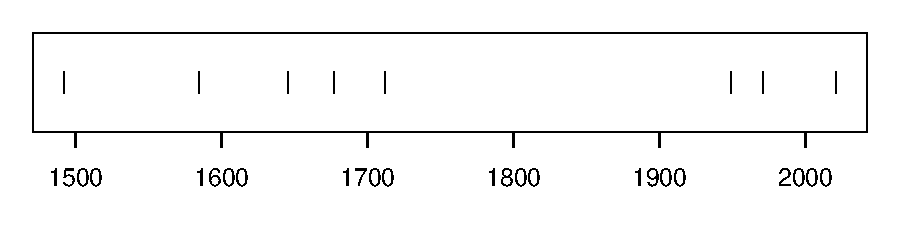
\includegraphics[keepaspectratio]{thesis_files/figure-latex/fig-timeline-1.pdf}}

}

\caption{\label{fig-timeline}Timeline of recent earthquakes on La Palma}

\end{figure}%

\textsubscript{Source:
\href{https://VJMeyer.github.io/submission/thesis.qmd.html}{Article
Notebook}}

\textsubscript{Source:
\href{https://VJMeyer.github.io/submission/thesis.qmd.html}{Article
Notebook}}

Based on data up to and including 1971, eruptions on La Palma happen
every 79.8 years on average.

Studies of the magma systems feeding the volcano, such as Marrero et al.
(2019), have proposed that there are two main magma reservoirs feeding
the Cumbre Vieja volcano; one in the mantle (30-40km depth) which
charges and in turn feeds a shallower crustal reservoir (10-20km depth).

Eight eruptions have been recorded since the late 1400s
(Figure~\ref{fig-timeline}).

Data and methods are discussed in Section~\ref{sec-data-methods}.

Let \(x\) denote the number of eruptions in a year. Then, \(x\) can be
modeled by a Poisson distribution

\begin{equation}\phantomsection\label{eq-poisson}{
p(x) = \frac{e^{-\lambda} \lambda^{x}}{x !}
}\end{equation}

where \(\lambda\) is the rate of eruptions per year. Using
Equation~\ref{eq-poisson}, the probability of an eruption in the next
\(t\) years can be calculated.

\begin{longtable}[]{@{}ll@{}}
\caption{Recent historic eruptions on La
Palma}\label{tbl-history}\tabularnewline
\toprule\noalign{}
Name & Year \\
\midrule\noalign{}
\endfirsthead
\toprule\noalign{}
Name & Year \\
\midrule\noalign{}
\endhead
\bottomrule\noalign{}
\endlastfoot
Current & 2021 \\
Teneguía & 1971 \\
Nambroque & 1949 \\
El Charco & 1712 \\
Volcán San Antonio & 1677 \\
Volcán San Martin & 1646 \\
Tajuya near El Paso & 1585 \\
Montaña Quemada & 1492 \\
\end{longtable}

Table~\ref{tbl-history} summarises the eruptions recorded since the
colonization of the islands by Europeans in the late 1400s.

\begin{figure}

\centering{

\pandocbounded{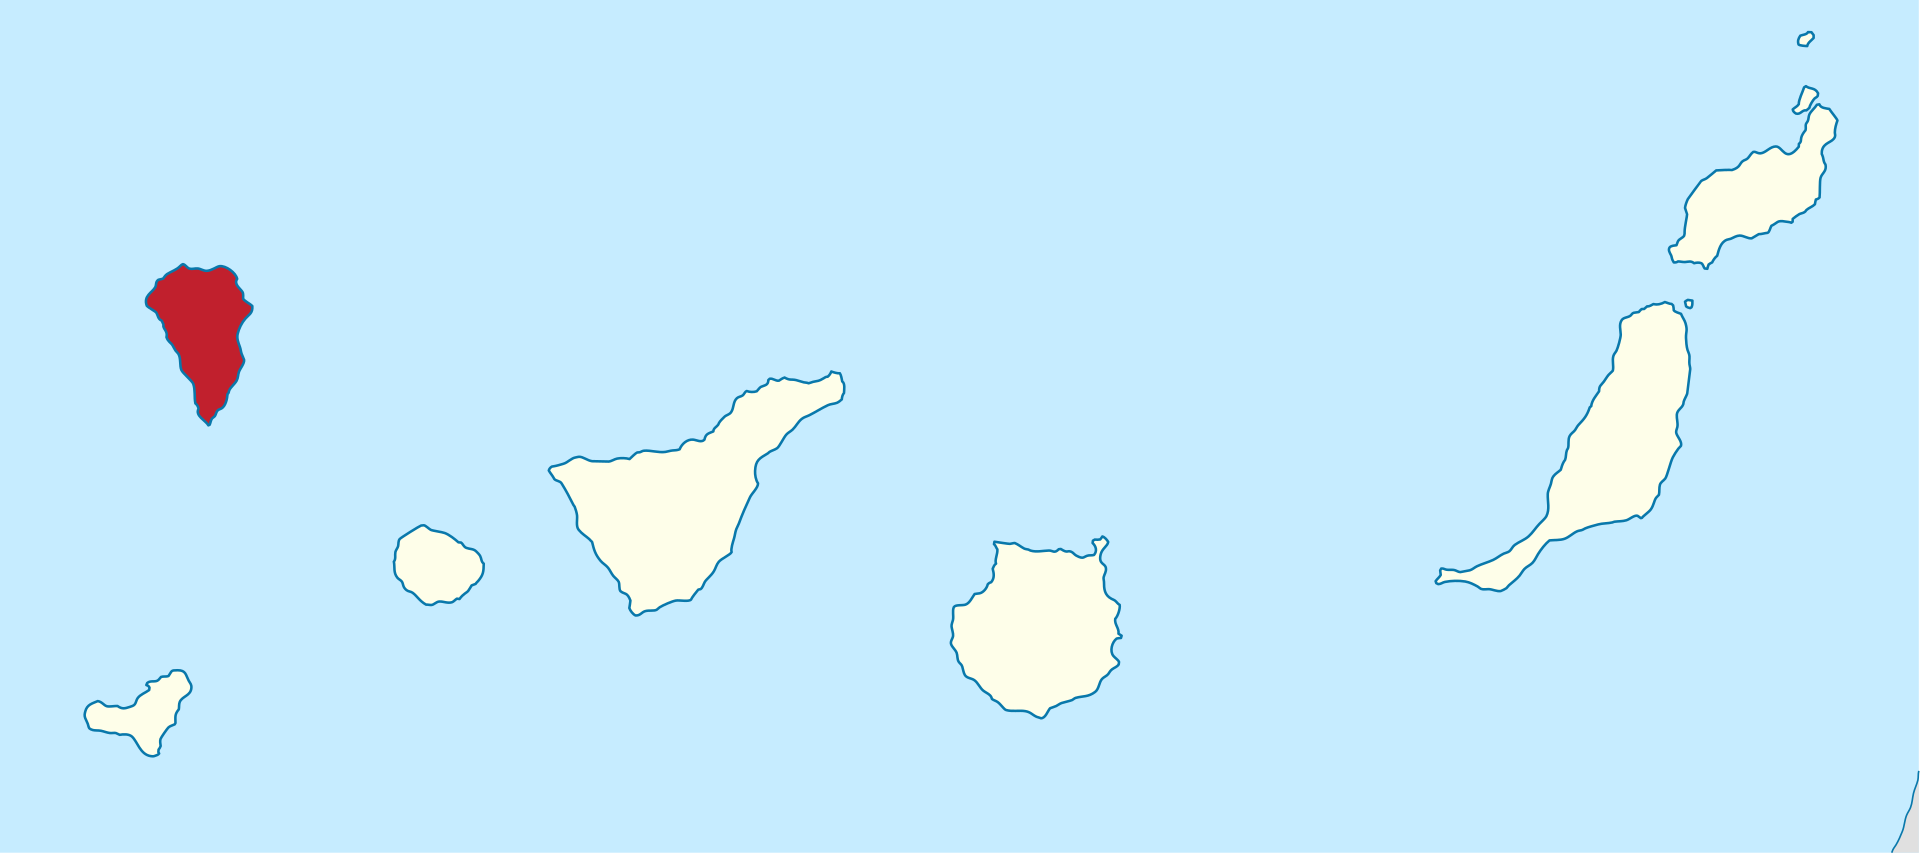
\includegraphics[keepaspectratio]{images/la-palma-map.png}}

}

\caption{\label{fig-map}Map of La Palma}

\end{figure}%

La Palma is one of the west most islands in the Volcanic Archipelago of
the Canary Islands (Figure~\ref{fig-map}).

\begin{figure}[H]

\centering{

\pandocbounded{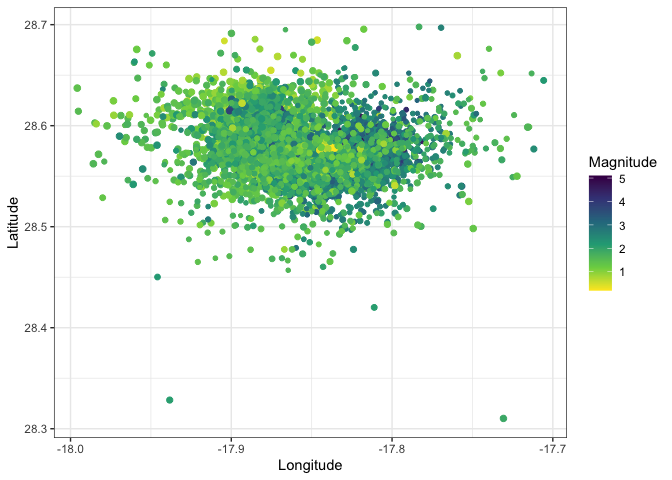
\includegraphics[keepaspectratio]{thesis_files/figure-latex/notebooks-explore-earthquakes-fig-spatial-plot-output-1.png}}

}

\caption{\label{fig-spatial-plot}Locations of earthquakes on La Palma
since 2017}

\end{figure}%

\textsubscript{Source:
\href{https://VJMeyer.github.io/submission/notebooks/explore-earthquakes.qmd.html\#cell-fig-spatial-plot}{Explore
Earthquakes}}

Figure~\ref{fig-spatial-plot} shows the location of recent Earthquakes
on La Palma.

\section{Data \& Methods}\label{sec-data-methods}

\section{Conclusion}\label{conclusion-1}

\chapter{Introduction}\label{introduction-2}

This is a booooook created from markdown and executable code.

See {[}Knuth (1984){]} and Knuth (1984) for additional discussion of
literate programming.

Regular markdown and \(E=mc^2\) equations.

\section{Quarto}\label{quarto}

Quarto enables you to weave together content and executable code into a
finished document. To learn more about Quarto see
\url{https://quarto.org}.

\section{Running Code}\label{running-code}

When you click the \textbf{Render} button a document will be generated
that includes both content and the output of embedded code. You can
embed code like this:

\begin{verbatim}
2
\end{verbatim}

You can add options to executable code like this

\begin{verbatim}
4
\end{verbatim}

The \texttt{echo:\ false} option disables the printing of code (only
output is displayed).

\begin{verbatim}
2
\end{verbatim}

More markdown.

\section{ToDo's}\label{todos}

// Double slash creates a new task

\textsubscript{Source:
\href{https://VJMeyer.github.io/submission/chapters/section1.qmd.html\#5c9cd77a-e4ad-4e45-8208-7fc2a66e21c3}{Introduction}}




\end{document}
